\section{Date: 2026-09-30}
\noindent \textbf{Series ID: IEAMSIPN} 

\noindent This series is titled Imports of Services: Charges for the use of intellectual property n.i.e. and has a frequency of Quarterly. The units are Millions of Dollars and the seasonal adjustment is Not Seasonally Adjusted.The observation start date is 1999-01-01 and the observation end date is 2026-04-01.The popularity of this series is 1. \\ 

\noindent \textbf{Series ID: DDURRE1A156NBEA} 

\noindent This series is titled Shares of gross domestic product: Personal consumption expenditures: Durable goods and has a frequency of Annual. The units are Percent and the seasonal adjustment is Not Seasonally Adjusted.The observation start date is 1929-01-01 and the observation end date is 2025-01-01.The popularity of this series is 4. \\ 

\subsection{Raw Regression}
\noindent Regresses the two series against each other directly. A significant result here can come just as easily from both series sharing a long-run trend as from any real relationship.

\begin{center}
\begin{tabular}{lclc}
\toprule
\textbf{Dep. Variable:}        & value\_fred\_DDURRE1A156NBEA & \textbf{  R-squared:         } &     0.321   \\
\textbf{Model:}                &             OLS              & \textbf{  Adj. R-squared:    } &     0.294   \\
\textbf{Method:}               &        Least Squares         & \textbf{  F-statistic:       } &     11.82   \\
\textbf{Date:}                 &       Wed, 30 Sep 2026       & \textbf{  Prob (F-statistic):} &  0.00206    \\
\textbf{Time:}                 &           17:05:45           & \textbf{  Log-Likelihood:    } &   -25.239   \\
\textbf{No. Observations:}     &                27            & \textbf{  AIC:               } &     54.48   \\
\textbf{Df Residuals:}         &                25            & \textbf{  BIC:               } &     57.07   \\
\textbf{Df Model:}             &                 1            & \textbf{                     } &             \\
\textbf{Covariance Type:}      &          nonrobust           & \textbf{                     } &             \\
\bottomrule
\end{tabular}
\begin{tabular}{lcccccc}
                               & \textbf{coef} & \textbf{std err} & \textbf{t} & \textbf{P$> |$t$|$} & \textbf{[0.025} & \textbf{0.975]}  \\
\midrule
\textbf{const}                 &       8.7930  &        0.314     &    28.002  &         0.000        &        8.146    &        9.440     \\
\textbf{value\_fred\_IEAMSIPN} &      -0.0001  &     3.39e-05     &    -3.438  &         0.002        &       -0.000    &    -4.67e-05     \\
\bottomrule
\end{tabular}
\begin{tabular}{lclc}
\textbf{Omnibus:}       &  5.919 & \textbf{  Durbin-Watson:     } &    0.272  \\
\textbf{Prob(Omnibus):} &  0.052 & \textbf{  Jarque-Bera (JB):  } &    1.819  \\
\textbf{Skew:}          &  0.005 & \textbf{  Prob(JB):          } &    0.403  \\
\textbf{Kurtosis:}      &  1.729 & \textbf{  Cond. No.          } & 2.36e+04  \\
\bottomrule
\end{tabular}
%\caption{OLS Regression Results}
\end{center}

Notes: \newline
 [1] Standard Errors assume that the covariance matrix of the errors is correctly specified. \newline
 [2] The condition number is large, 2.36e+04. This might indicate that there are \newline
 strong multicollinearity or other numerical problems.

\begin{figure}
\centering
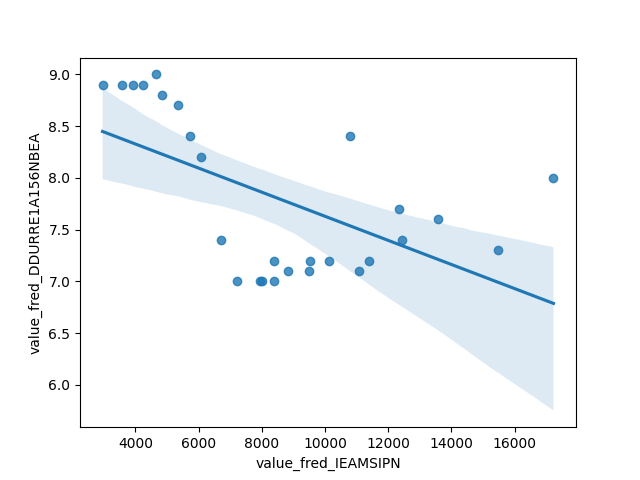
\includegraphics[scale = 0.9]{plots/plot_2026-09-30.png}
\caption{Raw Regression Plot for 2026-09-30}
\end{figure}
\newpage
\subsection{Detrended Regression}
\noindent Regresses the residuals of each series after removing its own linear time trend, so a shared trend can no longer drive the result on its own. A relationship that stays significant here is better evidence of a genuine link between the two series.

\begin{center}
\begin{tabular}{lclc}
\toprule
\textbf{Dep. Variable:}                   & value\_fred\_DDURRE1A156NBEA\_detrended & \textbf{  R-squared:         } &     0.024   \\
\textbf{Model:}                           &                   OLS                   & \textbf{  Adj. R-squared:    } &    -0.015   \\
\textbf{Method:}                          &              Least Squares              & \textbf{  F-statistic:       } &    0.6106   \\
\textbf{Date:}                            &             Wed, 30 Sep 2026            & \textbf{  Prob (F-statistic):} &    0.442    \\
\textbf{Time:}                            &                 17:05:45                & \textbf{  Log-Likelihood:    } &   -23.256   \\
\textbf{No. Observations:}                &                      27                 & \textbf{  AIC:               } &     50.51   \\
\textbf{Df Residuals:}                    &                      25                 & \textbf{  BIC:               } &     53.10   \\
\textbf{Df Model:}                        &                       1                 & \textbf{                     } &             \\
\textbf{Covariance Type:}                 &                nonrobust                & \textbf{                     } &             \\
\bottomrule
\end{tabular}
\begin{tabular}{lcccccc}
                                          & \textbf{coef} & \textbf{std err} & \textbf{t} & \textbf{P$> |$t$|$} & \textbf{[0.025} & \textbf{0.975]}  \\
\midrule
\textbf{const}                            &    6.162e-14  &        0.115     &  5.38e-13  &         1.000        &       -0.236    &        0.236     \\
\textbf{value\_fred\_IEAMSIPN\_detrended} &    8.159e-05  &        0.000     &     0.781  &         0.442        &       -0.000    &        0.000     \\
\bottomrule
\end{tabular}
\begin{tabular}{lclc}
\textbf{Omnibus:}       &  0.623 & \textbf{  Durbin-Watson:     } &    0.358  \\
\textbf{Prob(Omnibus):} &  0.732 & \textbf{  Jarque-Bera (JB):  } &    0.652  \\
\textbf{Skew:}          & -0.067 & \textbf{  Prob(JB):          } &    0.722  \\
\textbf{Kurtosis:}      &  2.250 & \textbf{  Cond. No.          } & 1.10e+03  \\
\bottomrule
\end{tabular}
%\caption{OLS Regression Results}
\end{center}

Notes: \newline
 [1] Standard Errors assume that the covariance matrix of the errors is correctly specified. \newline
 [2] The condition number is large, 1.1e+03. This might indicate that there are \newline
 strong multicollinearity or other numerical problems.

\begin{figure}
\centering
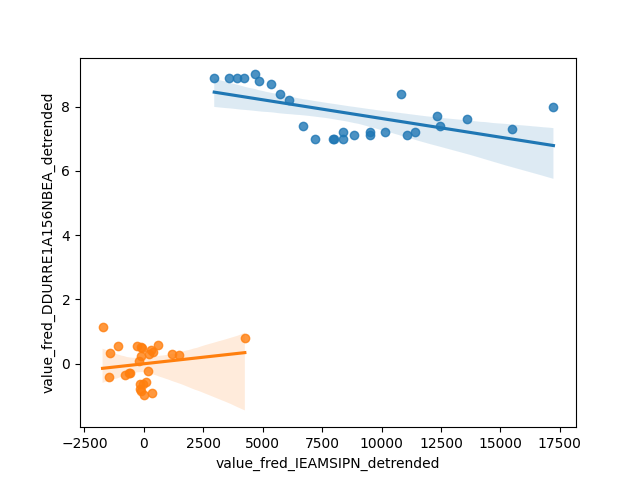
\includegraphics[scale = 0.9]{plots/plot_2026-09-30_detrended.png}
\caption{Detrended Regression Plot for 2026-09-30}
\end{figure}
\newpage
